 \documentclass{report}
 
\usepackage[utf8]{inputenc} 
\usepackage[T1]{fontenc}      
\usepackage[top=2.0cm, bottom=3cm, left=3.0cm, right=3.0cm]{geometry}
\usepackage{graphicx}
\usepackage{wrapfig}
\usepackage{amsmath,esint }
\usepackage{amssymb}
\graphicspath{{figures/}{../figures}}

\newcommand*\dif{\mathop{}\!\mathrm{d}}
\newcommand*\diver{\mathop{}\!\mathrm{div}}
\newcommand*\grad{\mathop{}\!\mathrm{grad}}

\begin{document}

\section*{Dimensionnement d'un aimant}

\begin{itemize}

	\item[$\heartsuit$] On commence par écrire les relations décrivant le milieu : respectivement Maxwell-Ampère, la conservation du flux de $\vec{B}$ et la relation caratéristique du milieu :
		\begin{align*}
		\begin{cases}
        	 H_al_a+H_fl_f+H_el_e=0 \\ 
			S_eB_e=S_aB_a=B_fl_f \\
			B_f = \mu_0\mu_{r,f}H_f\\
			B_e=\mu_0H_e
		\end{cases}  
		\end{align*}

\textit{NB : } Il n'y a pas de bobinage, donc pas d'excitation due à l'extérieur. Seule reste dans Maxwell-Ampère l'excitation originelle de l'aimant.

Il y a \textit{a priori} plusieurs façons d'arriver au résultat, de mon côté, j'exprime le champ magnétique dans l'entrefer $B_e$, fixé, en fonction des autres variables :
\begin{align}	
	B_e &=- \frac{\mu_0}{e}(H_al_a+H_fl_f)\\
	&=-\frac{\mu_0}{e}\left( H_al_a+\frac{B_f}{\mu_0\mu_{r,f}}l_f\right) \\
	&=-\frac{\mu_0}{e}\left( H_al_a+\frac{B_A}{\mu_0\mu_{r,f}}l_f\right) 
\end{align}

Or le terme $\frac{B_a}{\mu_0\mu_{r,f}}l_f$ est négligeable devant $B_e$ : cela revient à comparer $\frac{S_a}{S_e}$ et $\frac{l_f}{e\mu_{r,f}}$, et d'après l'hypothèse faite dans l'énoncé, $\frac{l_f}{e\mu_{r,f}}$ est négligeable.

On a donc : 
\begin{align*}
	& B_e =-\frac{\mu_0H_al_a}{e} \\
	\Leftrightarrow \quad & B_aB_e =-\frac{\mu_0B_aH_al_a}{e} \\
	\Leftrightarrow \quad & \frac{S_ee}{S_a}B_e^2 =-\mu_0B_aH_al_a \\
	\Leftrightarrow \quad & V_eB_e^2 =-\mu_0B_aH_aV_a \\
\end{align*}
	
	Comme les termes de gauches sont fixés, minimiser $V_a$ revient à maximiser $-B_aH_a$.

	\item[$\heartsuit$] Le produit $B_aH_a$ correspond à l'aire du carré $A(H)$ sous la courbe $(H,B(H))$. Pour le maximiser :
	\begin{align*}
		& A'(h)=0 \\
		\Leftrightarrow \quad & -\frac{d(B_aH_a)}{dH_a}=0 \\
		\Leftrightarrow \quad &0=-H_a\frac{d(B_a)}{dH_a}-B_a \\
		\Leftrightarrow \quad & \left|\frac{d(B_a)}{dH_a}\right|= \left|\frac{B_a}{H_a}\right|
	\end{align*}
	Le terme de droite représente la pente de la tangente à la courbe au point $P$, le premier terme le rapport $PI/IO$. Cela impose l'égalité des angles $(QI,QP)$ et $(OI,OP)$ et donc le caractère isocèle du triangle $OPQ$.
	
	\item[$\heartsuit$] Au point $P$, on lit : $B_a$ =0.40T et $H_a$ = 350kA/m, ce qui impose un volume :
	\begin{align*}
		V_a = \frac{V_eB_e^2}{\mu_0B_aH_a}=55\mathrm{cm}^3
	\end{align*}
Avec la conservation du flux, on a $S_a=B_eS_e/B_a=13,5\mathrm{cm}^2$. La longueur est alors $l_a=V_a/S_a = 4.1$cm.

\end{itemize}

\section*{Estimation de la puissance  dissipée dans un cycle hystérésis}

La puissance dissipée s'écrit comme $P=f\times \mathrm{Volume}\times \mathrm{Aire\ du\ cycle}$. L'aire peut être grossièrement assimilée à un rectangle d'aire $2\times75\mathrm{A/m}\times2\times0.75$T. On en déduit $P\approx2.4\times10^2$W. La puissance est dissipée en énergie thermique. 

\section*{Transformateur réel série}

\begin{itemize}
	
	\item[$\ast$] L’idée consiste à transférer les impédances du primaire au secondaire en les multipliant par le rapport de transformation au carré :
	\begin{align*}
		Z_{R_2}=(R_2+m^2R_1)+j\omega(L'_2+m^2L'_1)
	\end{align*}
	On rappelle que "passer" une impédance de l'autre côté du transformateur équivaut à multiplier celle-ci par $m^2$.
	
	\item[$\ast$] Lorsque le secondaire est court-circuité à 50 Hz, on a ce circuit :
	
\begin{figure}[h!]
	\centering
		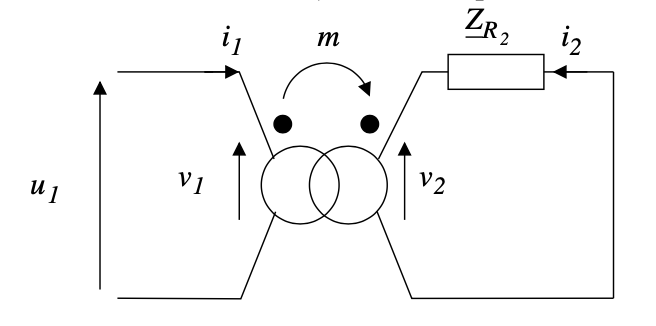
\includegraphics[scale=0.45]{transfo_reel_corr.png}
\end{figure}		

	\item[$\ast$] A ce moment-là, on a $u_{1cc}=v_1=\frac{v_2}{m}=-\frac{Z_{R_2}i_2}{m}$, donc :
	\begin{align*}
		U_{1cc}=\frac{|Z_{R_2}|I_{2cc}}{m}
	\end{align*}
	
	Le transformateur central étant idéal, la puissance fournie par le générateur est intégralement fournie au secondaire. La puissance est dissipée au secondaire dans les résistances, ce qui donne :
	\begin{align*}
		P_{1cc}=\frac{1}{2}(R_2+m^2R_1)I_{2cc}^2
	\end{align*}
	Le facteur 1/ provient qu'on est ici sur la puissance moyenne.
	
 Les formules théoriques obtenues sont des relations linéaires. L'ordonnée à l'origine des courbes expérimentales s'explique par les défauts non pris en compte : inductance de fuite pour la figure 1, pertes fer pour la figure 2,...	

	\item[$\ast$] On utilise les pentes pour déterminer les différentes grandeurs demandées.
	\begin{itemize}
	
		\item[-] figure 1 : la pente est l’inverse du rapport de transformation ($i_2=-i_1/m$), donc $m=0.5$	
		\item[-] Comme $R_2 =m R_1$, $P_{1cc}=m^2R_1I_{2cc}^2$, donc $R_1=\mathrm{pente}/m^2=8,8\Omega$
		
		\item[-] figure 2 : la relation entre $U_{1cc}$ et $I_{2cc}$ prend la forme simplifiée :
		\begin{align*}
			U_{1cc}=\frac{\sqrt{(2m^2R_1)^2+(2m^2L'_1)^2}}{m}I_{2cc}
		\end{align*}				
		On peut en déduire $L'_1+63$mH en l'isolant.
	\end{itemize}
		
	\end{itemize}

\section*{Transformateur réel}

\begin{itemize}

	\item[$\triangleright$] En négligeant la chute de tension due à la résistance des enroulements (modèle du transformateur parfait), pour le primaire :
	\begin{align*}
		v=-e=\frac{d\phi}{dt}=\frac{d(N_1B\times 2s)}{dt}=2sN_1j\omega B
	\end{align*}
	Pour les amplitudes, on obtient : 
	\begin{align*}
		V_{eff}\sqrt{2}=2\pi fN_1\times2sB_0 \quad \Leftrightarrow \quad N_1=\frac{V_{eff}\sqrt{2}}{2\pi f\times2sB_0}
	\end{align*}
On trouve $N_1=620$ spires. De la même manière pour avoir une tension 2$\times$ plus faible pour obtenir $V_2$, on trouve $N_2=310$.
Avec uen fréquence de 400 Hz, on trouve $N_1=78$ spires.

	\item[$\triangleright$] On applique Maxwell-Faraday et Maxwell-Ampère :
	\begin{align*}
		\begin{cases}
        	v_1=-e_1=\frac{d\phi_T}{dt}=j\omega N_1\phi \\ 
			v_2 = j\omega N_2\phi \\
			 N_1i_1+N_2i_2=H\times l=\frac{B}{\mu_0\mu_r}=\frac{\phi l}{\mu_0\mu_r S}
		\end{cases}  
	\end{align*}
	
	En remplaçant l'expression du flux, on obtient $N_1i_1+N_2i_2=\frac{v_1}{j\omega N_1}\times\frac{l}{\mu_0\mu_r S}$. En divisant par $N_1$, on obtient :
	\begin{align*}
		i_1-\frac{v_1}{j\omega \mu_0\mu_r SN_1^2/l}=-\frac{N_2}{N_1}i_2
	\end{align*}
	avec $L_1=\mu_0\mu_rN_1^2S/l$.
	
	\item[$\triangleright$] Pour $\mu_r\longrightarrow\infty$, $I_m\longrightarrow0$, cad on retrouve la loi de transformation des courants du transformateur idéal.

	\item[$\triangleright$] D'après $i_1 - I_m = - i_2$, on constate que la relation de transformation des courants s'applique en remplaçant $i_1$ par $i1 - I_m$, un courant $I_m$ est prélevé ; de la relation entre $I_m$ et $v_1$, on en déduit la présence en parallèle d'une inductance $L_1$ parcourue par le courant $I_m$.
	
	\item[$\triangleright$] $I_m=\frac{V_1}{2\pi fL_1}=73$mA.

\end{itemize}

\section*{Pic de courant dans un relais à palette}

\begin{itemize}
	
	\item[$\diamond$] La première étape consiste à déterminer l'inductance propre du dispositif qui permettra de déterminer l'énergie magnétique et la force magnétique ainsi que l'équation électrique. À section constante, la conservation du flux magnétique et l'absence de fuite magnétique impose $B=B_e=B_f$. On applique le théorème d'Ampère à l'excitation magnétique sur un contour incluant le matériau ferromagnétique et l'entrefer :
	\begin{align*}
		H_f\times l+H_e\times2x(t)=Ni(t)
	\end{align*}
Avec $B_f=\mu_0\mu_rH_f$ et $B_e=\mu_0H_e$, on en déduit :
\begin{align*}
	B = \frac{\mu_0Ni(t)}{l/\mu_r+2x(t)}
\end{align*}
	On peut alors en déduire le flux propre à travers les $N$ spires : 
\begin{align*}
	\phi = NBS = \frac{\mu_0N^2S}{l/\mu_r+2x(t)}i(t) \quad\Rightarrow L = \frac{\mu_0N^2S}{l/\mu_r+2x(t)}
\end{align*}	
	On applique la relation fondamentale de la dynamique à la palette. Une fois le support horizontal quitté, la palette est soumise à son poids et à la force électromagnétique, ce qui donne en projection sur l'axe vertical descendant :
\begin{align*}
	m\frac{d^2x}{dt^2}=mg+\left(\frac{\partial \varepsilon_m}{\partial x} \right)_{i=cste}=mg+\frac{1}{2}\frac{dL(x)}{dx}i^2 
\end{align*}	
	C'est-à-dire :
	\begin{align*}
		m\frac{d^2x}{dt^2}=mg- \frac{\mu_0N^2Si^2}{(l/\mu_r+2x)^2}
	\end{align*}
	
D'autre part, pour l'équation électrique on a un phénomène d'induction dans le bobinage :
\begin{align*}
	U=Ri-e=Ri+\frac{d(Li)}{dt}=Ri+i\frac{dL}{dt}+L\frac{di}{dt}=Ri+i\frac{dL}{dx}\frac{dx}{dt}+L\frac{di}{dt}
\end{align*} 
C'est-à-dire :
\begin{align*}
	U=Ri+\frac{\mu_0N^2S}{l/\mu_r+2x}\times\left[\frac{di}{dt} - \frac{2i}{l/\mu_r+2x}\frac{dx}{dt}\right] 
\end{align*}
On est bien en présence d'un système d’équations différentielles couplées.

	\item[$\diamond$] 1 : montée du courant. Dans un premier temps, le courant doit croître dans le circuit afin de créer une force électromagnétique suffisante pour compenser le poids et permettre à la palette de monter.
On peut donc considérer dans un premier temps que la distance $x$ reste fixée à $e$ et le circuit électrique est un simple circuit $RL_0$ qui subit un échelon de tension avec une constante de temps :
\begin{align*}
	\tau_0=\frac{L_0}{R}=\frac{\mu_0N^2S}{R(l/\mu_r+2e)}\simeq7\mathrm{ms}
\end{align*}
	Ceci semble cohérent avec la montée initiale du courant en quelques dixièmes de seconde et une immobilité mécanique.
	
2 : Seconde étape : mouvement mécanique. 
Sous l’effet de la force électromagnétique, la palette vient coller à l’aimant en U ; la baisse du courant peut s’interpréter comme une conséquence de la loi de Lenz, le système réagissant en tentant de contrer l’effet qui lui a donné naissance.

Troisième étape : seconde montée du courant
On se trouve à nouveau en présence d’un simple circuit $RL_1$ avec une inductance $L1$ > $L0$ et une constante de temps :
\begin{align*}
	\tau_1=\frac{L_1}{R}=\frac{\mu_0N^2S}{Rl/\mu_r}\simeq84\mathrm{ms}
\end{align*}
\end{itemize}

\section*{Transformateur à 3 bobinages}

\begin{itemize}
	\item[$\clubsuit$] On utilise les hypothèses du transformateur parfait. Le théorème d'Amplère s'écrit :
	\begin{align*}
		HL=N_1i_1+N_2i_2+N'_2i'_2
	\end{align*}
	Pour chaque spire $k$, Maxwell-Faraday s'écrit :
	\begin{align*}
		e_k=-j\omega\phi_{k}
	\end{align*}
	La conservation du flux impose : $\phi_{k}=N_k\phi_B$ et donc :
	\begin{align*}
		\frac{u_1}{N_1}=\frac{u_2}{N_2}=\frac{u'_2}{N'_2}
	\end{align*}	
	
	\item[$\clubsuit$] Si le transformateur est parfait, $HL=\frac{BL}{\mu_0\mu_r}\simeq0$. On a alors $N_1i_1+N_2i_2+N'_2i'_2=0$
	
\end{itemize}

\section*{Transfert de puissance}

On souhaite alimenter un dipôle ohmique de résistance $R$ par un générateur sinusoïdal de fem $e(t) = E_{0} cos(\omega t)$ par l'intermédiaire d'un transformateur supposé parfait de rapport de transmission $m$. Les câbles électriques reliant le transformateur ont un coefficient d'auto-induction $L$ et l'ensemble générateur-fils une résistance $r$.

\begin{itemize}
	\item[$\bigstar$] Déterminer le rapport de transformation pour avoir la puissance maximale dissipée dans $R$.
	\item[$\bigstar$] Calculer le rendement de l'installation électrique en fonction de $m$.
	\item[$\bigstar$] Tracer les courbes de la puissance dissipée dans $R$ en fonction de $m$.
\end{itemize}

\end{document}